\documentclass
[printout]
% [handout]
{beamer}

\usepackage[utf8]{inputenc}
\usepackage{graphics}
\usepackage{newcent}
\usepackage[absolute,overlay]{textpos}
\usepackage{calc}
\usetheme{Goettingen}
\usecolortheme{beaver}
\title[Git Study Day 2\\Introduction]{Introduction to Git}
\subtitle{CAT\&DOG Git study 2013\\Day 2}
\author{Eon Jeong}
\date{\today}

\begin{document}

\begin{frame}
  \titlepage
\end{frame}

\setcounter{section}{-1}

\section{Contents}

\begin{frame}{Contents}
  \tableofcontents
\end{frame}

\setcounter{section}{0}

\section{Overview}

\begin{frame}
  \sectionpage
\end{frame}

\begin{frame}{Git, in comparison with Subversion}
  \begin{center}
    \begin{tabular}{c|cc}
      & \texttt{git} & \texttt{svn} \\\hline\hline\pause
      topology& \textit{distributed}& \textit{centralized}\\\hline
      configuration& one at top& all recursive\\\hline
      mergeable& everything& b2t only\\\hline
      objects stored& itself& difference\\\hline
      mg. method& 3-way& 2-way\\\hline
      temp. save& multiple& local copy?\\\hline
      commit id& hexadec. hash& serial dec. no.\\\hline\hline\pause
      on/offline& \multicolumn{2}{c}{only possible in git}\\\hline
      branch cost & \multicolumn{2}{c}{cheaper in git}\\\hline
      complexity & \multicolumn{2}{c}{svn costs less ideally}\\\hline
      performance & \multicolumn{2}{c}{git does much better}\\\hline
    \end{tabular}
  \end{center}
\end{frame}

\section{Beginning a local repository}

\begin{frame}
  \sectionpage
\end{frame}

\begin{frame}{\texttt{init}}
  Create an empty repository in current directory, or reinitialize an existing one.
\end{frame}

\begin{frame}{\texttt{commit}}
  Post a new revision from files in the workspace.
\end{frame}

\begin{frame}{\texttt{add}}
  Stage(index) some file(s) to be committed.
\end{frame}

\begin{frame}{\texttt{checkout}}
  Get file(s) from a specific revision to the workspace.
\end{frame}

\begin{frame}{\texttt{status}}
  Show status of the workspace.
\end{frame}

\begin{frame}{\texttt{log}}
  List commits from recent ones and their references.
\end{frame}

\section{Looking over GitHub}

\begin{frame}
  \sectionpage
\end{frame}

\begin{frame}{https://github.com}
  \begin{center}
    
\includegraphics[height=7.5cm]{github-unsigned.jpg}
  \end{center}
\end{frame}

\begin{frame}{https://github.com (signed in)}
  \begin{center}
    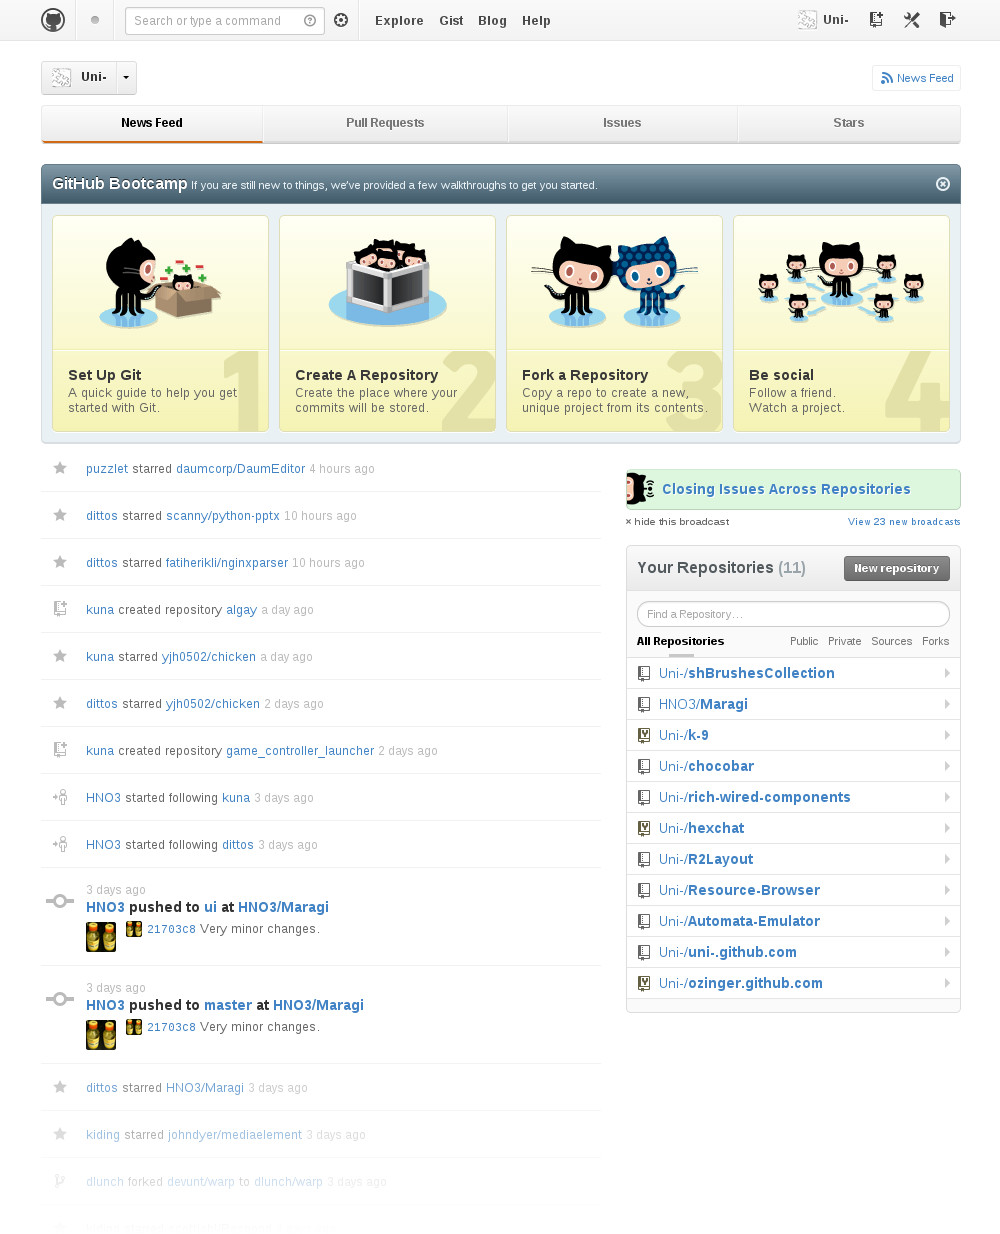
\includegraphics[height=7.5cm]{github-signed.jpg}
  \end{center}
\end{frame}

\begin{frame}{https://github.com/dittos/LonelyIsland}
  \begin{center}
    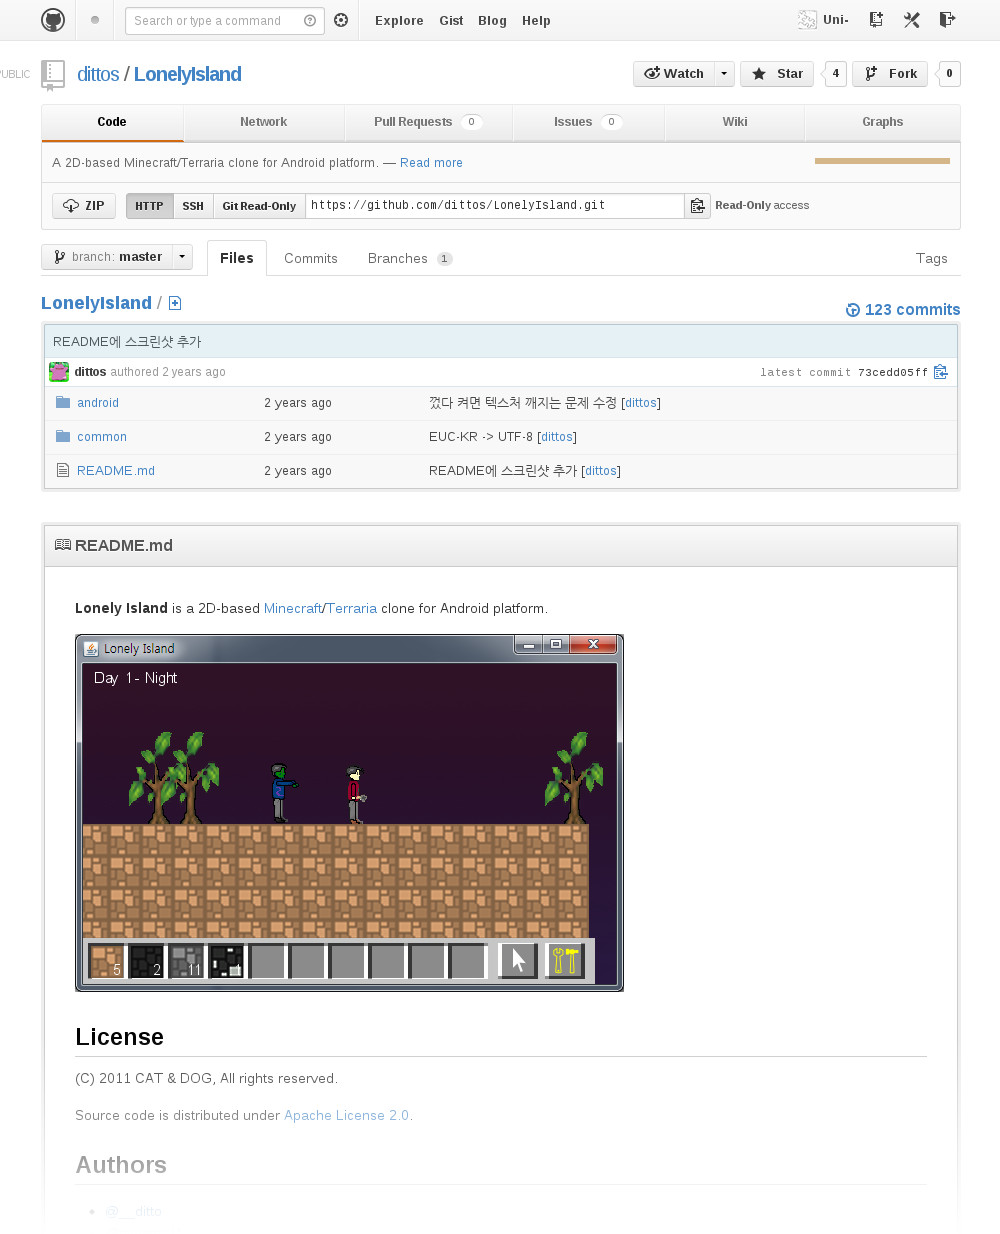
\includegraphics[height=7.5cm]{github-repo.jpg}
  \end{center}
\end{frame}

\begin{frame}{https://github.com/Uni-/studying-repo}
  How to create a GitHub repo\pause
  \begin{enumerate}
  \item Click "Create a new repo"
  \item Type name and description\pause
  \item ???
  \item PROFIT!
  \end{enumerate}
\end{frame}

\section{Interacting with remote repositories}

\begin{frame}
  \sectionpage
\end{frame}

\begin{frame}{\texttt{clone}}
  Make a repository into a new subdirectory, with remote \texttt{origin} and its brances.\pause\\
  Equivalent:
  \begin{itemize}
  \item (\texttt{mkdir}, \texttt{cd})
  \item \texttt{init}
  \item \texttt{remote add origin}
  \item \texttt{fetch origin}
  \item \texttt{checkout master}
  \end{itemize}
\end{frame}

\begin{frame}{\texttt{pull}}
  Apply a remote repository to the remote reference and attach branches to the corresponding upstream.\pause\\
  Equivalent:
  \begin{itemize}
  \item \texttt{fetch <remote>}
  \item \texttt{merge <branch>}
  \end{itemize}
\end{frame}

\begin{frame}{\texttt{push}}
  Update associated remote repositories and references, applying changes from the local one.
\end{frame}

\section{Assignment}

\begin{frame}{Second week's assignment}
  \begin{enumerate}
  \item \textbf{Let me gather all your names!}
    \begin{itemize}
    \item Fork \textit{Uni-/studying-repo}.
    \item Clone your fork on a local system.
    \item Append your name on the list in \texttt{README.md}.\\(Note: no necessity it is real one.)
    \item Make a commit and push to \textit{your} remote repo.\pause
    \item Write a pull request. \textit{(optional)}
    \end{itemize}
  \end{enumerate}
  \begin{textblock*}{2cm}[1.0, 0](\paperwidth, 0pt)
    
\includegraphics[height=2cm]{forkme.png}
  \end{textblock*}
\end{frame}

\end{document}
